\vspace{-2mm}
\section{Analysis}
\label{sec:analysis}
\vspace{-1mm}

\subsection{Choice of diffusion framework}
\label{subsec:diffusion_choice}
\vspace{-1mm}

As explained in Section \ref{sec:framework}, we could in principle use any diffusion model variant in our world model. While \textsc{diamond} utilizes \textsc{edm} \citep{karras2022elucidating} as described in Section \ref{sec:method}, \textsc{ddpm} \citep{ho2020DDPM} would also be a natural candidate, having been used in many image generation applications \citep{ldm_stable_diffusion, ddpm++}. We justify this design decision in this section.

To provide a fair comparison of \textsc{ddpm} with our \textsc{edm} implementation, we train both variants with the same network architecture, on a shared static dataset of 100k frames collected with an expert policy on the game \textit{Breakout}. As discussed in Section \ref{subsec:dwm_training}, the number of denoising steps is directly related to the inference cost of the world model, and so fewer steps will reduce the cost of training an agent on imagined trajectories. \citet{ho2020DDPM} use a thousand denoising steps, and \citet{ldm_stable_diffusion} employ hundreds steps for Stable Diffusion. However, for our world model to be computationally comparable with other world model baselines (such as \textsc{iris} which requires 16 NFE for each timestep), we need at most tens of denoising steps, and preferably fewer. Unfortunately, if the number of denoising steps is set too low, the visual quality will degrade, leading to compounding error. 

To investigate the stability of the diffusion variants, we display imagined trajectories generated autoregressively up to $t=1000$ timesteps in Figure \ref{fig:denoising_trajectories}, for different numbers of denoising steps $n \le 10$. We see that using \textsc{ddpm} (Figure \ref{fig:denoising_with_ddpm}) in this regime leads to severe compounding error, causing the world model to quickly drift out of distribution. In contrast, the \textsc{edm}-based diffusion world model (Figure \ref{fig:denoising_with_karras}) appears much more stable over long time horizons, even for a single denoising step. A quantitative analysis of this compounding error is provided in Appendix~\ref{app:ddpm_drift}.

% %%%%%%%%%%%%%%%%%%%%%%%
\begin{figure}[h]
  \begin{subfigure}{0.49\linewidth}
    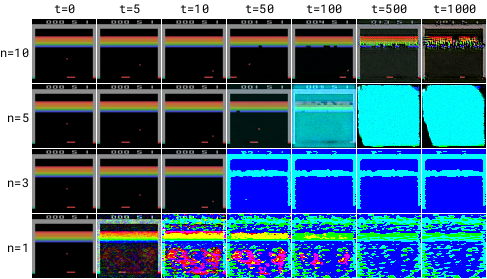
\includegraphics[width=\linewidth]{images/figure__karras_vs_ddpm__ddpm.png}
    \caption{\textsc{ddpm}-based world model trajectories.} \label{fig:denoising_with_ddpm}
  \end{subfigure}%
  \hspace*{\fill}   % maximize separation between the subfigures
  \begin{subfigure}{0.49\textwidth}
    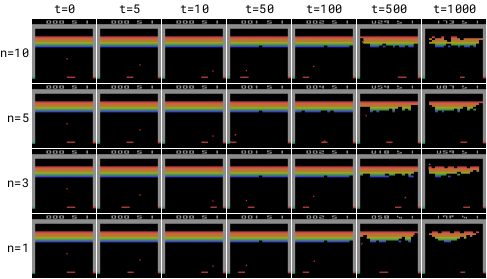
\includegraphics[width=\linewidth]{images/figure__karras_vs_ddpm__karras.png}
    \caption{\textsc{edm}-based world model trajectories.} \label{fig:denoising_with_karras}
  \end{subfigure}%

\caption{Imagined trajectories with diffusion world models based on \textsc{ddpm} (left) and \textsc{edm} (right). The initial observation at $t=0$ is common, and each row corresponds to a decreasing number of denoising steps $n$. We observe that \textsc{ddpm}-based generation suffers from compounding error, and that the smaller the number of denoising steps, the faster the error accumulates. In contrast, our \textsc{edm}-based world model appears much more stable, even for $n=1$.\vspace{-5mm}}
\label{fig:denoising_trajectories} 
\end{figure}
% %%%%%%%%%%%%%%%%%%%%%%%

This surprising result is a consequence of the improved training objective described in Equation~\ref{eq:effective_obj}, compared to the simpler noise prediction objective employed by \textsc{ddpm}. While predicting the noise works well for intermediate noise levels, this objective causes the model to learn the identity function when the noise is dominant ($\sigma_{noise}\gg\sigma_{data} \implies \xi_\theta(\x^\tau_{t+1}, y_t^\tau)\to\mathbf{x}^\tau_{t+1}$), where $\xi_\theta$ is the noise prediction network of \textsc{ddpm}. This gives a poor estimate of the score function at the beginning of the sampling procedure, which degrades the generation quality and leads to compounding error.

In contrast, the adaptive mixing of signal and noise employed by \textsc{edm}, described in Section \ref{subsec:practical_dwm}, means that the model is trained to predict the clean image when the noise is dominant ($\sigma_{noise}\gg\sigma_{data} \implies \mathbf{F_\theta}(\mathbf{x}^\tau_{t+1},y_t^\tau)\to\mathbf{x}^0_{t+1}$). This gives a better estimate of the score function in the absence of signal, so the model is able to produce higher quality generations with fewer denoising steps, as illustrated in Figure \ref{fig:denoising_with_karras}.


\subsection{Choice of the number of denoising steps}\label{subsec:denoising_steps}

 While we found that our \textsc{edm}-based world model was very stable with just a single denoising step, as shown for \textit{Breakout} in the last row of Figure \ref{fig:denoising_with_karras}, we discuss here how this choice would limit the visual quality of the model in some cases. We provide more a quantitative analysis in Appendix~\ref{app:denoising_ablation}.

As discussed in Section \ref{subsec:diffusion}, our score model is equivalent to a denoising autoencoder \citep{vincent2008extracting} trained with an $L_2$ reconstruction loss. The optimal single-step prediction is thus the expectation over possible reconstructions for a given noisy input, which can be out of distribution if this posterior distribution is multimodal. While some games like \textit{Breakout} have deterministic transitions that can be accurately modeled with a single denoising step (see Figure \ref{fig:denoising_with_karras}), in some other games partial observability gives rise to multimodal observation distributions. In this case, an iterative solver is necessary to drive the sampling procedure towards a particular mode, as illustrated in the game \textit{Boxing} in Figure \ref{fig:too_optimisitic_4_sure}. As a result, we therefore set $n=3$ in all of our experiments.
\vspace{-2mm}
%%%%%%%%%%%%%%%%%%%%%%%
\begin{figure}[h!]
%\vspace{-6mm}
\begin{center}
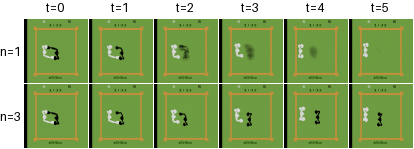
\includegraphics[width=.64\linewidth]{images/figure__blurry_boxing.png}
\caption{Single-step (top row) versus multi-step (bottom row) sampling in \textit{Boxing}. Movements of the black player are unpredictable, so that single-step denoising interpolates between possible outcomes and results in blurry predictions. In contrast, multi-step sampling produces a crisp image by driving the generation towards a particular mode. Interestingly, the policy controls the white player, so his actions are known to the world model. This information removes any ambiguity, and so we observe that both single-step and multi-step sampling correctly predict the white player's position.}
\label{fig:too_optimisitic_4_sure}
\end{center}
\vspace{-4mm}
\end{figure}
%%%%%%%%%%%%%%%%%%%%%%%


\subsection{Qualitative visual comparison with \textsc{iris}}
\label{subsec:comparison_transformers}

We now compare to \textsc{iris} \citep{iris2023}, a well-established world model that uses a discrete autoencoder \citep{vqvae} to convert images to discrete tokens, and composes these tokens over time with an autoregressive transformer \citep{radford2019language}. For fair comparison, we train both world models on the same static datasets of 100k frames collected with expert policies. This comparison is displayed in Figure \ref{fig:iris_vs_diamond} below.

% %%%%%%%%%%%%%%%%%%%%%%%
\begin{figure}[h]
  \begin{subfigure}{0.49\linewidth}
    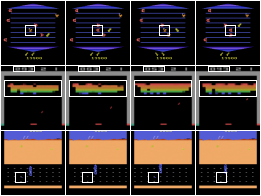
\includegraphics[width=\linewidth]{images/figure__iris_vs_diamond__iris.png}
    \caption{\textsc{iris}} \label{fig:iris_vs_diamond__iris}
  \end{subfigure}%
  \hspace*{\fill}   % maximize separation between the subfigures
  \begin{subfigure}{0.49\textwidth}
    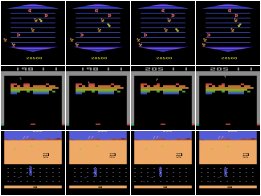
\includegraphics[width=\linewidth]{images/figure__iris_vs_diamond__diamond.png}
    \caption{\textsc{diamond}} \label{fig:iris_vs_diamond__diamond}
  \end{subfigure}%
\caption{Consecutive frames imagined with \textsc{iris} (left) and \textsc{diamond} (right). The white boxes highlight inconsistencies between frames, which we see only arise in trajectories generated with \textsc{iris}. In \textit{Asterix} (top row), an enemy (orange) becomes a reward (red) in the second frame, before reverting to an enemy in the third, and again to a reward in the fourth. In \textit{Breakout} (middle row), the bricks and score are inconsistent between frames. In \textit{Road Runner} (bottom row), the rewards (small blue dots on the road) are inconsistently rendered between frames. None of these inconsistencies occur with \textsc{diamond}. In \textit{Breakout}, the score is even reliably updated by +7 when a red brick is broken\protect\footnotemark.}
\label{fig:iris_vs_diamond}
\end{figure}

\footnotetext{\href{https://en.wikipedia.org/wiki/Breakout_(video_game)\#Gameplay}{\texttt{https://en.wikipedia.org/wiki/Breakout\_(video\_game)\#Gameplay}}}
% %%%%%%%%%%%%%%%%%%%%%%%

We see in Figure \ref{fig:iris_vs_diamond} that the trajectories imagined by \textsc{diamond} are generally of higher visual quality and more faithful to the true environment compared to the trajectories imagined by \textsc{iris}. In particular, the trajectories generated by \textsc{iris} contain visual inconsistencies between frames (highlighted by white boxes), such as enemies being displayed as rewards and vice-versa. These inconsistencies may only represent a few pixels in the generated images, but can have significant consequences for reinforcement learning. For example, since an agent should generally target rewards and avoid enemies, these small visual discrepancies can make it more challenging to learn an optimal policy.

These improvements in the consistency of visual details are generally reflected by greater agent performance on these games, as shown in Table \ref{tab:atari_results_full}. Since the agent component of these methods is similar, this improvement can likely be attributed to the world model. 

Finally, we note that this improvement is not simply the result of increased computation. Both world models are rendering frames at the same resolution ($64\times64$), and \textsc{diamond} requires only 3 NFE per frame compared to 16 NFE per frame for \textsc{iris}. This is further reflected by the fact that \textsc{diamond} has significantly fewer parameters and takes less time to train than \textsc{iris}, as provided in Appendix \ref{app:performance_profile}.